\section{SAC头段变量}
\label{sec:sac-header-variables}

\subsection{基本变量}

\subsubsection{\texttt{nvhdr}*}
SAC头段版本号。nvhdr\footnote{星号表示该头段变量在SAC中必须有定义值,下同。}是SAC中很重要但是不太常用的头段变量。
目前值为6,旧版本的SAC文件($nvhdr<6$)在读入时会自动更新。

\subsubsection{\texttt{nzyear, nzjday, nzhour, nzmin, nzsec, nzmsec}}
分别表示``年''、``一年的第几天''\footnote{使用jday而不是``month+day''可以少用一个
头段变量。}、``时''、``分''、``秒''、``毫秒''\footnote{$1 s = 1000 ms$}。
这六个头段变量构成了SAC中唯一的绝对时刻,SAC中的其它时刻都被转换为相对于该时刻的
相对时间(单位为秒)。详细的信息参见第~\ref{sec:sac-time}~节``~\nameref{sec:sac-time}~''中的
介绍。

根据这六个头段还可以推导出其它一些辅助型变量:
\begin{itemize}
\ttfamily
\item kzdate:字符数字格式的参考日期,由nzyear和nzjday导出;
\item kztime:字符数字格式的参考时间,由nzhour、nzmin、nzsec、nzmsec导出;
\end{itemize}

如下例所示:
\begin{SACCode}
SAC> fg seis
SAC> lh nzyear nzjday nzhour nzmin nzsec nzmsec
  
  FILE: SEISMOGR - 1
 --------------

     nzyear = 1981
     nzjday = 88
     nzhour = 10
      nzmin = 38
      nzsec = 14
     nzmsec = 0
SAC> lh kzdate kztime 
  
  FILE: SEISMOGR - 1
 --------------

     kzdate = MAR 29 (088), 1981
     kztime = 10:38:14.000
\end{SACCode}

\subsubsection{\texttt{iztype}}
等效参考时刻。SAC的参考时刻是可以任意指定的,但一般选取某个特定的时刻(比如
文件起始时刻、发震时刻等等)作为参考时刻。其可以取如下枚举值:
\begin{itemize}
\ttfamily
\item IUNKN:未知
\item IB:以文件开始时刻为参考时间
\item IDAY:以参考日期当天的午夜作为参考时间
\item IO:以事件发生时间为参考时间
\item IA:以初动到时为参考时间
\item ITn:以用户自定义的时间为参考时间(n可取0-9)
\end{itemize}

若iztype=IO,则表示其值以发震时刻作为参考时刻,此时头段变量o的值应为0。

\subsubsection{\texttt{iftype}*}
SAC文件类型,其决定了头段区之后有几个数据区。该头段变量为枚举类型
\footnote{枚举型在C源码中实际为``\lstinline{\#define ITIME 1}''的形式。}
,可以取如下几个枚举值
\footnote{枚举值一律使用大写,且以I开头。} :
\begin{itemize}
\ttfamily
\item ITIME:时间序列文件(即Y数据,一般的地震波形数据)
\item IRLIM:频谱文件(实部-虚部格式)
\item IAMPH:频谱文件(振幅-相位格式)
\item IXY:一般的X-Y数据
\item IXYZ:一般的XYZ(3-D)文件
\end{itemize}

\subsubsection{\texttt{idep}}
因变量(Y)类型,该头段变量可以不定义,其可以取如下枚举值:
\begin{itemize}
\ttfamily
\item IUNKN:未知类型
\item IDISP:位移量,单位为$nm$
\item IVEL:速度量,单位为$nm/s$
\item IVOLTS:速度量,单位为$volts$\footnote{不解}
\item IACC:加速度量:单位为$nm/s^2$	
\end{itemize}

\subsection{数据相关变量}
\subsubsection{\texttt{npts}*}
数据点数,其值决定了在数据区有多少个数据点。

\subsubsection{\texttt{delta}*}
等间隔数据的数据点采样周期(标称值)。

\subsubsection{\texttt{odelta}}
采样周期的实际值,若实际值与标称值不同则有值,一般来说都是未定义的。

\subsubsection{\texttt{b*, e*}}
文件的起始时间和结束时间(相对于参考时刻的相对时间)。

\subsubsection{\texttt{leven}*}
若数据为等间隔则为TRUE,否则为FALSE。

\subsubsection{\texttt{depmin, depmax, depmen}}
因变量(Y)的最小值、最大值和均值。一般地,这几个头段会在读/写SAC文件时、数据处理
过程中被自动计算。

\subsubsection{\texttt{scale}}
因变量比例因子,即真实物理场被乘以该比例因子而得到现有数据。比如真实物理场的Y值
大概在$10^{-20}$量级,数据处理起来很不方便,这个时候可以设置scale=$10^{20}$,
将真实物理场的量级修改到$10^1$。

\subsubsection{\texttt{xminimum, xmaximum, yminimum, ymaximum}}
仅用于3D(XYZ)文件中,记录X和Y的最小/大值。

\subsubsection{\texttt{nxsize, nysize}}
仅用于3D(XYZ)文件中,表示X和Y方向的数据点数。

\subsubsection{\texttt{iqual}\dag}
iqual\footnote{\dag 标识仅表示SAC程序内部未使用该头段变量,即变量有值或者无值、有何值,
对于程序的运行不会产生任何影响,但用户可以在自己的程序中自由使用这些头段变量。下同。
}
标识数据质量,可取如下值:
\begin{itemize}
\ttfamily
\item IGOOD:高质量数据;
\item IGLCH:数据中有毛刺(glitches);
\item IDROP:数据有丢失(Dropouts);
\item ILOWSN:低信噪比数据;
\item IOTHER:其它;
\end{itemize}

\subsubsection{\texttt{isynth}\dag}
合成数地震图标识。
\begin{itemize}
\ttfamily
\item IRLDTA:真实数据;
\item ??????:其它合成地震图代码相应的标识;
\end{itemize}

\subsection{事件相关变量}
\subsubsection{\texttt{kevnm}}
事件名。在头段区,其占据16个字节。

\subsubsection{\texttt{evla, evlo, evel, evdp}}
分别代表事件的纬度(-90到90)、经度(-180到180)、高程(单位为m,未使用)和
深度(单位为$km$,以前为$m$)。

\subsubsection{\texttt{ievreg}\dag}
事件地理区域\footnote{Flinn-Engdahl Regions:\url{http://en.wikipedia.org/wiki/Flinn-Engdahl_regions}}。

\subsubsection{\texttt{ievtyp}}
事件类型,这里仅列出部分常见的枚举值:
\begin{itemize}
\ttfamily
\item IUNKN:未知事件
\item INUCL:核事件
\item IEQ:地震
\item IOTHER:其它
\end{itemize}

\subsubsection{\texttt{mag}}
事件震级。

\subsubsection{\texttt{imagsrc}}
震级信息来源,可以取如下枚举值:
\begin{itemize}
\ttfamily
\item INEIC:\href{http://earthquake.usgs.gov/regional/neic/}{NEIC}
\item IPDE:\href{http://earthquake.usgs.gov/data/pde.php}{PDE}
\item IISC:\href{http://www.isc.ac.uk/}{ISC}
\item IREB:人工检查过的事件目录
\item IUSGS:\href{http://earthquake.usgs.gov}{USGS}
\item IBRK:\href{http://seismo.berkeley.edu/}{UC Berkeley}
\item ICALTECH:\href{http://www.seismolab.caltech.edu}{California Institute of Technology}
\item ILLNL:\href{https://www.llnl.gov/}{Lawrence Livermore National Laboratory}
\item IEVLOC:Event Location
\item IJSOP:Joint Seismic Observation Program
\item IUSER:The individual using SAC2000
\item IUNKNOWN:未知
\end{itemize}

\subsubsection{\texttt{imagtyp}}
震级类型,取如下枚举值:
\begin{itemize}
\ttfamily
\item IMB:体波震级
\item IMS:面波震级
\item IML:Local震级
\item IMW:矩震级
\item IMD:持续时间震级
\item IMX:用户自定义震级
\end{itemize}

\subsubsection{\texttt{gcarc, dist, az, baz}}
\begin{description}
\item [gcarc] 全称Great Circle Arc,即震中到台站的大圆弧的长度,单位为度;
\item [dist] 震中到台站的距离,单位为千米;
\item [az] 方位角,震中到台站的连线与地理北向的夹角;
\item [baz] 反方位角,台站到震中的连线与地理北向的夹角。
\end{description}

\begin{figure}[H]
\centering
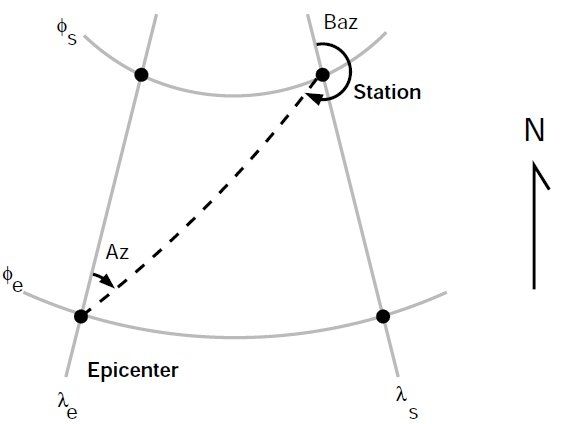
\includegraphics[width=8cm]{gcarc-dist-az-baz}
\caption[震中距、方位角、反方位角示意图]{震中距、方位角、反方位角示意图。图片来自于Prof. Robert B. Herrmann 的课程讲义。}
\label{fig:gcarc-dist-az-baz}
\end{figure}

震中距、方位角和反方位角的计算涉及到球面三角的知识,具体细节可以参考该讲义:\\
\scriptsize\url{http://www.eas.slu.edu/People/RBHerrmann/Courses/EASA462/ASSIGNMENTS/Ass07/Ass07.pdf}。

\normalsize
在不严谨的情况下,可以认为dist = gcarc*111.195,更严谨的计算方法可以参考相关文献。

知道震中和台站的位置,计算震中距、方位角和反方位角是一个基本问题,有很多代码均实现了
此功能,列举如下:
\begin{itemize}
\item \url{http://www.seis.sc.edu/software/distaz/}
\item SAC源码~\lstinline{src/ucf/distaz.c}
\item CPS330\footnote{\url{http://www.eas.slu.edu/eqc/eqccps.html}}源码~\lstinline{VOLI/src/udelaz.c}
\end{itemize}

\subsubsection{\texttt{o, ko}}
o为事件的发生时刻相对于参考时刻的秒数。ko是绘图时变量o的标识符。

\subsubsection{\texttt{khole}}
若为核爆事件,则其为孔眼标识;若为其它事件,则为位置标识。

\subsubsection{\texttt{nevid, norid, nwfid}}
三者分别标识事件ID、起始时间ID和波形ID,仅用于CSS 3.0文件中。CSS 3.0
是SAC可以处理的一种数据格式,应该是当初SAC商业化的产物,目前仍保留
在SAC头段中。

\subsection{台站相关变量}
\subsubsection{\texttt{knetwk}}
地震台网名。

\subsubsection{\texttt{kstnm}}
台站名。

\subsubsection{\texttt{istreg}\dag}
台站地理区域。

\subsubsection{\texttt{stla, stlo, stel, stdp}}
台站纬度(-90到90度)、经度(-180到180度)、高程(单位m,目前未使用)、
相对地表的深度(单位m,目前未使用)。

\subsubsection{\texttt{cmpaz, cmpinc, kcmpnm, kstcmp}}
一个台站至少需要三个正交的通道(或分量)才能完整地记录地面运动物理量。cmpaz和cmpinc
指定了单个通道记录的方向矢量。

图~\ref{fig:cmpaz-cmpinc}~给出了SAC所使用的NEU坐标系,需要注意的是这是一个左手坐标系。
图中蓝色箭头为通道所记录的方向矢量,若地面运动与该方向一致,则为正,否则为负。
其中,头段变量cmpaz表征通道的方位角,其定义为从N向开始顺时针旋转的角度,即图中的角度$\phi$;
cmpinc表征通道的入射角,定义为U向向下旋转的度数,即图中的角度$\theta$。

\begin{figure}[H]
\centering
\tdplotsetmaincoords{55}{50}
\pgfmathsetmacro{\rvec}{.8}
\pgfmathsetmacro{\thetavec}{30}
\pgfmathsetmacro{\phivec}{30}
\begin{tikzpicture}[scale=5,tdplot_main_coords]
\coordinate (O) at (0,0,0);
\draw[thick,->] (0,0,0) -- (1,0,0) node[anchor=south west]{$E$};
\draw[thick,->] (0,0,0) -- (0,1,0) node[anchor=south]{$N$};
\draw[thick,->] (0,0,0) -- (0,0,1) node[anchor=north east]{$U$};

\tdplotsetcoord{P}{\rvec}{\thetavec}{\phivec}
\draw[-stealth,color=blue] (O) -- (P);
\draw[dashed, color=red] (O) -- (Pxy);
\draw[dashed, color=red] (P) -- (Pxy);

\tdplotdrawarc{(O)}{0.2}{\phivec}{90}{anchor=west}{$\phi$}

\tdplotsetthetaplanecoords{\phivec}
\tdplotdrawarc[tdplot_rotated_coords]{(0,0,0)}{0.5}{0}%
{\thetavec}{anchor=south west}{$\theta$}
\end{tikzpicture}
\caption{cmpaz和cpminc示意图}
\label{fig:cmpaz-cmpinc}
\end{figure}

根据定义,地震仪标准通道的cmpinc和cmpaz值如下表:
\begin{table}[H]
\caption{标准地震通道的cmpaz和cpminc}
\label{table:neu-cmpaz-cmpinc}
\centering
\begin{tabular}{ccc}
\toprule
方向    &   CPMAZ   &   CPMINC      \\
\midrule
N       &   0       &   90          \\
E       &   90      &   90          \\
U       &   0       &   0           \\
\bottomrule
\end{tabular}
\end{table}

对于非标准方向的地震通道来说,很容易根据cmpinc和cmpaz的值,将其旋转到NEU坐标系或者
RTZ坐标系,这些将在``~\nameref{sec:traces-rotating}~''一节中说到。

kcmpnm为分量名称,SEED格式规定使用三个字符中的最后一个字符代表通道的方位(如BHE代表东西向分量)。
对于水平分量,目前更趋向于使用1和2代替N和E。

kstcmp为辅助型变量,表示台站分量,由kstnm、cmpaz、cmpinc推导得到。

\subsubsection{\texttt{lpspol}}
如图~\ref{fig:cmpaz-cmpinc}~所示,SAC使用左手坐标系NEU,若台站三通道的正极性分别与
NEU三方向相同,则为真,否则为假。

\subsection{震相相关变量}
\subsubsection{\texttt{a, ka, f, kf}}
a和f分别为事件的初动时刻和结束时刻相对于参考时刻的秒数。ka和kf则是相应的时间标识。

\subsubsection{\texttt{tn, ktn}}
用户自定义的时刻,n可以取0-9,常用于震相拾取,ktn为相应的时间标识。
比如定义t1为PcP震相的到时,kt1则一般定义为``PcP''。

\subsection{仪器相关变量}
\subsubsection{\texttt{kinst}, \texttt{iinst}\dag, \texttt{respn}\dag}
kinst为记录仪器的通用名称,iinst为记录仪器的类型,respn为仪器相应参数。

\subsection{其它变量}
\subsubsection{\texttt{usern, kusern}}
usern(n=0-9)和kusern(n=0-2)均用来存储用户自定义值。不像a和ka那样成对存在,
usern和kusern之间没有对应关系。比如可以将波形的信噪比保存在user0中,将任意字符串
保存到kuser0中。

\subsubsection{\texttt{lovrok}}
若为真,则数据可覆盖;若为假,则数据不可被覆盖。主要用于保护原始数据,一般来说
很少用到,若是出于保护原始数据的目的,应优先考虑对原始数据做备份。

\subsubsection{\texttt{lcalda}}
全称为Calculate Dist and Azimuth,若为真,则在事件和台站的坐标被写入或被修改时,
dist、gcarc、az、baz将自动计算。

\subsubsection{\texttt{kdatrd}}
数据被读入计算机的日期。
